\subsection{(n,r,s)-граф}

\begin{lemma}
	Имеют место следующие 2 утверждения:
	\begin{enumerate}
		\item \(C_n^k \le \frac{n^k}{k!}\)
		
		\item \(C_n^k = \frac{n^k}{k!} \exp \ps{-\frac{k(k - 1)}{2n} + O(k^3 / n^2)}\)
	\end{enumerate}
\end{lemma}

\begin{proof}
	Распишем биномиальный коэффициент, как мы это сделали в доказательстве теоремы:
	\[
		C_n^k = \frac{n!}{k! (n - k)!} = \frac{n(n - 1) \ldots (n - (k - 1))}{k!} = \frac{n^k}{k!} \prod_{t = 0}^{k - 1} \ps{1 - \frac{t}{n}} \le \frac{n^k}{k!}
	\]
	Для второго надо расписать натуральный логарифм через формулу Тейлора с О-большим:
	\begin{multline*}
		C_n^k = \frac{n^k}{k!} \exp\ps{\sum_{t = 0}^{k - 1} \ln\ps{1 - \frac{t}{n}}} = \frac{n^k}{k!} \exp\ps{\sum_{t = 0}^{k - 1} \ps{-\frac{t}{n} + O\ps{\frac{t^2}{n^2}}}} =
		\\
		\frac{n^k}{k!} \exp\ps{-\frac{k(k - 1)}{2n} + O\ps{\frac{k^3}{n^2}}}
	\end{multline*}
	Дополнительное пояснение: а почему мы имеем право так сложить О-большие? Потому что все логарифмы разложены по формуле Тейлора в нуле (формула Маклорена), то есть коэффициенты одинаковы. Мы их просто выносим для нужных слагаемых и получаем ответ.
\end{proof}

\begin{corollary}~
	\begin{itemize}
		\item Если $k = k(n) = o(\sqrt{n})$, то имеет место эквивалентность:
		\[
			C_n^k \sim \frac{n^k}{k!}
		\]
		
		\item Если $k^3 = o(n^2)$, то имеет место другая эквивалентность:
		\[
			C_n^k \sim \frac{n^k}{k!} \cdot e^{-\frac{k(k - 1)}{2n}}
		\]
	\end{itemize}
\end{corollary}

\begin{theorem} (Формула Стирлинга, без доказательства)
	Для факториала верна следующая эквивалентность:
	\[
		n! \sim \sqrt{2\pi n} {(\frac{n}{e})}^n
	\]
\end{theorem}

\begin{theorem}
	Если $k = \floor{an}$, где $a \in (0; 1)$, то для биномиальных коэффициентов справедлива следующая эквивалентность:
	\[
		C_n^{\floor{an}} \sim (a^{-a}(1 - a)^{-(1 - a)} + o(1))^n
	\]
\end{theorem}

\begin{proof}
	Начнём аккуратно расписывать биномиальный коэффициент через формулу Стирлинга:
	\begin{multline*}
		C_n^{\floor{an}} = \frac{n!}{\floor{an}! (n - \floor{an})!} \sim
		\\
		\sqrt{2\pi n} \ps{\frac{n}{e}}^n \cdot \frac{1}{\sqrt{2\pi \floor{an}}} \ps{\frac{e}{\floor{an}}}^{\floor{an}} \cdot \frac{1}{\sqrt{2\pi (n - \floor{an})}} \ps{\frac{e}{n - \floor{an}}}^{n - \floor{an}} =
		\\
		n^n \underbrace{\frac{\sqrt{2\pi n}}{\sqrt{2\pi \floor{an}} \cdot \sqrt{2\pi (n - \floor{an})}}}_{\Pi(n)} \cdot \frac{1}{(\floor{an})^{\floor{an}}} \cdot \frac{1}{(n - \floor{an})^{n - \floor{an}}}
	\end{multline*}
	Если бы могли как-то избавиться от округлений, то можно было бы сократить $n^n$. А что, идея хорошая: давайте распишем округление как $\floor{an} = an - \eps_n,\ \eps_n \in [0; 1)$. Тогда
	\begin{multline*}
		C_n^{\floor{an}} \sim n^n \Pi(n) \frac{1}{(an - \eps_n)^{an - \eps_n}} \cdot \frac{1}{(n - an + \eps_n)^{n - an + \eps_n}} =
		\\
		\Pi(n) \frac{n^n}{(an)^{an - \eps_n} \cdot (n - an)^{n - an + \eps_n}} \cdot \frac{1}{\ps{1 - \frac{\eps_n}{an}}^{an - \eps_n} \cdot \ps{1 + \frac{\eps_n}{n - an}}^{n - an + \eps_n}} =
		\\
		\Pi(n) Q(n) \cdot \frac{n^n}{(an)^{an} (n - an)^{n - an}} = \Pi(n) Q(n) \cdot \ps{a^{-a} (1 - a)^{-(1 - a)}}^n
	\end{multline*}
	Остаётся доказать, что 2 коэффициента спереди не вносят вклад в эквивалентность. Для этой цели, вернёмся к исходной формуле и покажем такую равносильность (для простоты записи обозначим $A = a^{-a}(1 - a)^{-(1 - a)}$):
	\[
		C_n^{\floor{an}} \sim (A + o(1))^n \Longleftrightarrow \ln C_n^{\floor{an}} \sim n\ln(A)
	\]
	\begin{itemize}
		\item ($\Ra$) Обозначим $o(1) = \delta \to 0$. Тогда
		\[
			\ln C_n^{\floor{an}} = n\ln(A + \delta) = n\ln A + n\ln(1 + \delta/A)
		\]
		Из условия $\ln(1 + \delta/A)$ тоже стремится к нулю. Стало быть
		\[
			\lim_{n \to \infty} \frac{n\ln A + n\ln(1 + \delta / A)}{n \ln A} = 1
		\]
		
		\item ($\La$) Условие означает, что
		\[
			\lim_{n \to \infty} \frac{\ln C_n^{\floor{an}}}{n\ln(A)} = 1 \Lra \ln C_n^{\floor{an}} = n\ln(A) + o(1)
		\]
		\textcolor{red}{Не придумал}
	\end{itemize}
	Значит, нужно проверить такую эквивалентность:
	\[
		\ln C_n^{\floor{an}} \sim \ln(\Pi(n)Q(n)A^n) \sim n\ln(A)	
	\]
	Действительно, $\ln(\Pi(n)Q(n)A^n) = \ln(\Pi(n)) + \ln(Q(n)) + n\ln(A)$
	\begin{itemize}
		\item То, что мы обозначили за $\Pi(n)$, является $O(n)$. Стало быть, $\ln(\Pi(n)) = O(\ln n) = o(n)$
		
		\item Аккуратно разберёмся с каждым сомножителем, входящим в $Q(n)$:
		\[
			\ln\ps{\frac{1}{(an)^{-\eps_n}}} = \eps_n \ln(an) = o(n); \quad \ln\ps{\frac{1}{(n - an)^{\eps_n}}} = -\eps_n \cdot \ln(n - an) = o(n)
		\]
		И другие 2:
		\[
			\ps{1 - \frac{\eps_n}{an}}^{\eps_n - an} \xrightarrow{} 1 \cdot e^{-\eps_n} = o(n); \quad \ps{1 - \frac{\eps_n}{n - an}}^{n - an + \eps_n} \xrightarrow{} e^{-\eps_n} \cdot 1 = o(n)
		\]
		
		\item $\ln(A^n) = n\ln(A)$. Тут, думаю, пояснений не надо.
	\end{itemize}
	Таким образом
	\[
		\lim_{n \to \infty} \frac{\ln(\Pi(n)) + \ln(Q(n)) + n\ln(A)}{n\ln(A)} = 1
	\]
\end{proof}

\begin{definition}

Определим $G(n,r,s)$ следующим образом:

\begin{itemize}
    \item $V = \{A \subset \{1,2,\dots,n\}:|A|=r\}$
    \item $E=\{(A,B): |A \cap B| = s\}$
\end{itemize}


То есть это граф, вершинами которого являются всевозможные $r$-элементные подмножества. Две вершины соединяем ребром, если соответствующие множества пересекаются ровно по $s$ элементам.

\end{definition}

\begin{example}
При $n = 5, r = 2, s = 0$ получится граф Петерсена.

\end{example}

\begin{definition}
    Граф называется регулярным, если степени всех его вершин равны.
\end{definition}

\begin{example}
Рассмотрим $G(n, \frac{n}{2}, \frac{n}{4})$.
Чему равна степень каждой вершины? Для этого нам нужно посчитать, сколько существует $\frac{n}{2}$-элементных подмножеств, пересекающихся с данным по $\frac{n}{4}$ элементам. Их ${({{C_{\frac{n}{2}}}^{\frac{n}{4}}})}^2$, потому что мы должны выбрать $\frac{n}{4}$ элементов из нашего множества, и $\frac{n}{4}$ из оставшихся элементов, не лежащих в нашем множестве. Значит, $|E| = \frac{1}{2}C_n^{\frac{n}{2}}{({{C_{\frac{n}{2}}}^{\frac{n}{4}}})}^2$.\\
Посчитаем теперь количество треугольников в таком графе. Для этого зафиксируем две вершины, соединённые ребром и посчитаем, сколько есть вершин, которые соединены с каждой из наших:

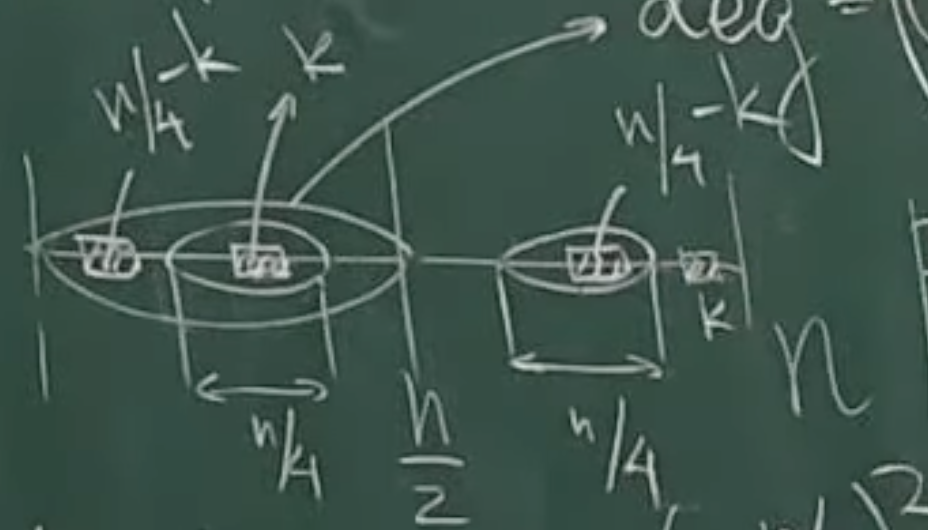
\includegraphics[width=0.8\textwidth]{images/lecture2_nrs.png}

Первая вершина - это левая ''сарделька'', а вторая - объединение сардельки внутри первой и сардельки справа. Вершина, которую мы выбираем, должна пересекаться с обеими вершинами по $\frac{n}{4}$ элементам. Давайте выберем $k$ элементов из пересечения первой и второй вершины. Тогда из оставшейся части первой сардельки нужно выбрать $\frac{n}{4} - k$. Так как вершина - это $\frac{n}{2}$-элементное множество, осталось выбрать туда еще $\frac{n}{4}$ элементов. Чтобы было ребро со второй вершиной, нужно выбрать еще $\frac{n}{4} - k$ из правой маленькой сардельки. Выберем теперь из оставшейся части всего множества еще $k$ элементов и получим вершину, которая удовлетворяет требованиям. Всего получаем $C_\frac{n}{4}^k C_\frac{n}{4}^{\frac{n}{4}-k} C_\frac{n}{4}^{\frac{n}{4}-k} C_\frac{n}{4}^{k} = (C_{\frac{n}{4}}^k)^4$ способов. Значит, число треугольников можно посчитать по формуле: 

\[
T_3 = (\sum_{k=0}^{\frac{n}{4}} (C_{\frac{n}{4}}^k)^4) \cdot \frac{1}{6}\cdot C_n^{\frac{n}{2}} (C_{\frac{n}{2}}^{\frac{n}{4}}) ^2
\]
\begin{definition}
    Матрицей Адамара называется матрица $n \times n $, элементами которой являются $\pm 1$, обладающая следующим свойством: любые две строки и любые два столбца ортогональны. 
\end{definition}

\begin{definition}
    Кликой в графе называется любой его полный подграф.
\end{definition}

%%\textcolor{red}{дописать про связь с матрицами Адамара} 
\end{example}

\subsection{Клики, независимые множества, хроматические числа}

\begin{definition}
	\textit{Кликовым числом} графа $G = (V, E)$ называется максимальный размер клики в этом графе:
	\[
		w(G) = \max_{W \subseteq G \text{ --- клика}} |W|
	\]
\end{definition}

\begin{definition}
	Пусть $G = (V, E)$ --- произвольный граф. Тогда подмножество $W \subseteq V$ называется \textit{независимым}, если выполнено условие:
	\[
		\forall x, y \in W\ (x, y) \notin E
	\]
\end{definition}

\begin{definition}
	\textit{Числом независимости} графа $G = (V, E)$ называется максимальный размер среди всех его независимых множеств:
	\[
		\alpha(G) = \max_{W \subseteq G \text{ --- независимое}} |W|
	\]
\end{definition}

\begin{definition}
	\textit{Хроматическим числом} графа $G = (V, E)$ называется минимальное число цветов, которыми можно покрасить вершины графа так, что у любого ребра концы будут разноцветными.
	
	Для формального описания, введём множество функций-раскрасок:
	\[
		\mathcal{C} = \{\chi \colon V \to \N \mid \forall (x, y) \in E\ \chi(x) \neq \chi(y)\}
	\]
	Тогда хроматическое число можно записать так:
	\[
		\chi(G) = \min_{\chi \in \mathcal{C}} | \chi(V)|
	\]
\end{definition}

\begin{note}
	Мы используем букву $\chi$ из-за ассоциации с латинским словом chroma, обозначающим цвет.
\end{note}

\begin{example}
Пусть $C_n$ - простой цикл на $n$ вершинах. Тогда \[ \chi(C_n) = \begin{cases}
    2, n=2k\\
    3, n = 2k + 1\\
\end{cases}\]

\end{example}

\begin{proposition}
$\chi(G) = 2$ тогда и только тогда, когда в $G$ нет нечётных циклов. Такой граф называется двудольным.
\end{proposition}